
\chapter{Optimizing Temporal Rule-Based Classification}
\label{Chap:Optimizing}

\section{Introduction}

This chapter answers the question posed in chapter one regarding the players' classification in the Public Goods Game data sets. The aim is to compare the Optimizing Temporal Rule-Based Classification proposed in chapter three section  \ref{sec:Temporal-Rule-Based-Classification} against the available classification method which is used by economists \cite{Fischbacher2001}. This comparison is formed into a Hypothesis \ref{hypo:proposedClassification} in chapter one. If this hypothesis holds true, this means our proposed method is performing better than the available classification method.

After classifying players with the proposed method, we use their new classes to answer two more questions about players behaviour. The first question concerns consistency of players strategy in various length of the game. To answer this question, we will check the validity of Hypothesis \ref{hypo:lengthOftheGame} as it states that the length of the game does not affect player strategy. The second question concerns using the overall general behaviour as Reference of Behaviour as our Hypothesis \ref{hypo:overallBehavoiur} in chapter one states that using overall behaviour as a reference of behaviour is more stable than the other two methods; the first time point and the previous time point. If this hypothesis holds true, so measuring changes over time can be performed reliably regardless of the underlying clustering and external cluster validity indices.

 

Hypothesis \ref{hypo:proposedClassification} indicates that using flexible rules by experts and then later optimising and specifying these rules will generate classes which are more representative of player's behaviour during the game. While this hypothesis is specific about the domain of the data set namely a public goods game, the proposed classification method can, however, be used on data sets with similar properties.  For example, stock market price data, students' performance over the years and effects of drugs on patients. In chapter six, we will classify stock market data using the proposed classification method.

The proposed classification method has two main steps. The first step uses specific definitions from field experts for classes which exist for items. These definitions are based on aggregated attributes of the temporal data. The second step is the optimisation process. In this step, the best possible classifier for the items will be selected. The best classifier is a classifier which can produce the most compacted classes of items (players) at each time point in the temporal data. The compactness of the classes is calculated by using a cost function which is based on the overall dispersal of items in each class. Classes' dispersal can be measured by using internal cluster validity indices like the Dunn Index, distance measures like Euclidean distance or statistical measures such as standard deviation.

In this chapter, we use brute force to find the best classifier. Brute force is simple and can solve classification in a relatively reasonable time for the available public goods game data sets. However, it can not perform optimally with a larger amount of data. Therefore, in the next chapter, we will replace the brute force with a heuristic method, namely differential evolutionary algorithm DEA, to optimise rules of the classifier.


\section{Background}
Most rule-based classifications use the  'if..else..' form to classify underlying data, which is conducive for easier comprehension  \cite{Negnevitsky2002}. The rules can be learned through examples or provided by an expert \cite{Wang1992}. As explained below, many different data mining and analysis methods use rule-based systems for classification. 

Rule-based classifications are used in fuzzy systems. For example Cordon et al. \cite{Cordon1999} proposed a new Fussy Reasoning Method (FRM) with better optimisation for the system, whereby the rules do not lose their comprehensibility. Ishibuchi \cite{Ishibuchi1999} compared two kinds of voting schemes for fuzzy rule-based classification.

Experts use common sense and vague terms to solve problems and classify situations/items, while an expert system that tries to simulate human experts uses logic to conclude decisions instead of hard programmed solutions \cite{Negnevitsky2002}. A number of expert systems that rely on rule-based logic have been introduced \cite{Styvaktakis2002}.

Many other methods have been introduced that use rule-based systems for classification, like \cite{Giacometti2008}, which proposed a generic classifier construction algorithm (ICCA). \cite{Qin2009} proposed an algorithm for a rule-based classifier that can extract rules from uncertain data, and used probability estimation for rule learning, inspired by the use of probabilities to construct decision trees.

To classify players in the public goods data sets, economists use players' contribution tables \cite{Fischbacher2001}. In this table, players state their intent for contribution in response to the rounded average contribution of other co-players. Thus, this table consists of players intended contribution conditioned by the contribution of other players ranging from 0 to 20. According to the players' response, economists classify them into four classes which are conditional co-operator, free riders, triangle contributors and others.

However, classifying players according to the contribution table which has been completed by the players prior to the game rounds might not represent players' actual behaviour during the game. This table ignores players' real contribution in the game rounds, which might change during games due to the change in their strategy as a result of their experience from previous game rounds.

There are many well known temporal classification methods which use either dynamic time warping \textbf{DTW} \cite{Berndt1994} or Euclidean distance to classify time series data sets. Examples of temporal classifiers such as Douzal-Chouakria et al. \cite{Douzal-Chouakria2012} used decision trees, Vincent S. Tseng et al. used Naive Bayes sequence classifier \cite{Tseng2009} and Ranganatha Sitaram et al. used  Support Vector Machine \textbf{SVM} as a temporal classifier with different kernels \cite{Sitaram2007}. However, all these methods require training set samples which are necessary to build their classifier instead of following experts definition to classify items in the temporal data. 

The available data sets for public goods games do not contain labels for players that reflect their behaviour during the game because experts use contribution tables to classify players. However, these tables are not directly related to their behaviour. Using a static contribution table is easier for economists to classify players as they can follow players answers manually or using simple methods. This simplified method can not be done with the temporal data even though it better reflects player behaviour. In chapter two, multiple examples are presented for methods of extracting rule-based classifiers using genetic  \cite{McAulay1994}, evolutionary algorithms \cite{Orriols-Puig2009} and SVM \cite{Nunez2006}. However, these methods require training data sets to build the classifier. 
 

\section{Approach}

The proposed classification method consists of two main steps; rule generation and rule optimisation, as shown in figure  \ref{fig:classificationProcess}. The optimised rules can be reconstructed as a decision tree.  As explained in chapter two, decision trees and rule-based classifiers can interchangeably represent each other. However, rule-based representation is preferable to humans as they are more intuitive and they might also be more efficient than their counterparts of decision trees.

In the subsections below we will detail the process of the rule generation and the methods of determining the number of classes and limits of each class. Then, we discuss the optimisation process and the parameters which are to be optimised as well as methods for measuring the optimum classifier such as using internal cluster validity indices and Euclidean distance among items. Finally, we will lay out a comparison method between the results of the proposed classification method and available classification for players of the public goods game.

\begin{figure}[!h]
    \centering
    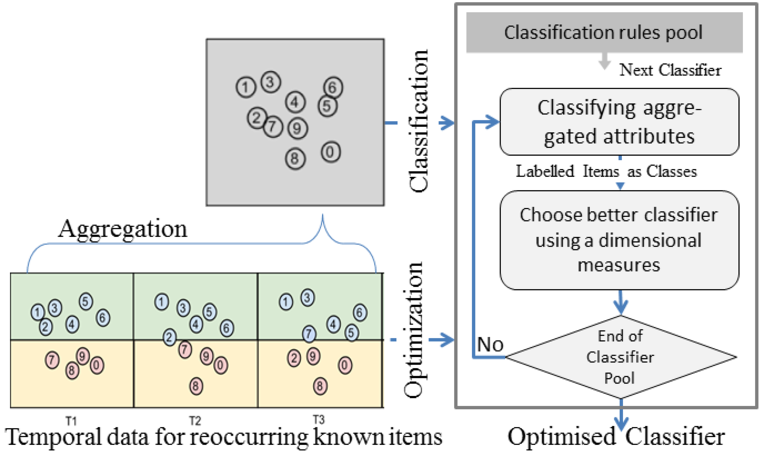
\includegraphics[width=0.9\textwidth]{images/chapter5/classificationProcess.png}
    \caption{An illustration of the proposed classification algorithm and its relation with temporal data and their aggregates.}
    \label{fig:classificationProcess}
\end{figure}


\subsection{Choosing Initial Limits for Classes}
\label{sec:Choosing_Initial_Limits_for_Classes}
For a selected number of classes, every class has a limit in each of the aggregated (non-temporal) attributes which are used in the classification rules. A limit is start and end values of a class of a certain attribute or dimension, and these can be represented by [min, max] pairs. As we mentioned in chapter three section \ref{sec:Generating-Initial-Rules}, classification rules are formulated in a nested if-else fashion to evaluate items' class as well as classes of priorities. The class limits for the attributes are represented in the if conditions of the classification rules using logical operations like $\leqslant and \geqslant$. 

A general template for class rules is shown in algorithm \ref{alg:PrioritizingTheClasses}. The classes priority is embedded through multi if-else statements. In the practical implementation,  for the sake of clarity and simplicity, the rule of each class can be represented in a method which returns $true$ value if the attributes of an instance satisfy the conditions of the class or $false$ otherwise. The last branch of the nested statement can be one of these options:
\begin{itemize}
    \item An else statement which represents a class with extreme values which can always be satisfied after all other classes are tested
    \item An else statement which represents ''others'' or elements which can not be classified by the given set of rules. 
    \item An elseif statement represents one of the classes. In this case, any outlier with extreme values will be ignored and not classified.
\end{itemize}

\begin{algorithm}[!h]
    \SetAlgoLined
    \If{Conditions for Class A}{
        Item is class A;
    }
    \ElseIf{Conditions for Class B}{
        Item is class B;
    }
    \ElseIf{Conditions for Class C}{
        Item is class C;
    }
    \Else{
        Item is Class Others;
    }
    \caption{Simple Multi if-else statements to priorities classes}
    \label{alg:PrioritizingTheClasses}
\end{algorithm}

To produce initial rules for classes with their range of values for each class limit in the aggregated attributes, the knowledge of experts in the specific field is required. However, experts might need specific types of aggregated attributes which should be created to formulate these rules. Moreover, to visualise data as an aid for the human expert to make more informed decisions about the class rules, an item profile should be created. In later subsections, we will discuss the methods of formulating rules through human experts, data manipulation and item profiling.

\subsubsection{Data Manipulation}

The final classification rules are expressed in the form of aggregated attributes or any available static (none-temporal) attributes. These aggregated attributes are derived from temporal attributes of the available items in the data set. Each items' temporal attribute can be aggregated in many ways as required by the classification rules. Possible aggregations for temporal attributes can be originated from basic statistical analyses such as:

\begin{itemize}
    \item \textbf{Total:} Returns the summation of all available time points' values.
    \item \textbf{Mean:} Returns the total of a temporal attribute divided by the number of time points.
    \item \textbf{Median:} Returns the middle value of a temporal attribute after sorting all values of the available time points.
    \item \textbf{Mode:} Returns the most frequent value from available time points of a temporal attribute.    \item \textbf{Count:} The occurrence number (frequency) of a value or targeted values. For example, the number of zero contribution in all rounds for each player in public goods games or the number of failed subjects for each student in the entirety of their study.
    \item \textbf{Minimum:} Returns the lowest value of a temporal attribute among all values of the available time points.
    \item \textbf{Maximum:} Returns the highest value of a temporal attribute among all values of the available time points.
\end{itemize}

\begin{table}[!h]
    \ra{1.3}
    \small
    \centering
    \caption{Sample of the public goods game data with three aggregated  attributes which are derived from temporal attributes. The aggregated attribute headers are denoted by their respective mathematical notation.}
    \label{tab:CreatingAggrigations}
    \begin{tabular}{ccccccc}
        \toprule
        Player ID & Time & Belief & Contribution & \textbf{$\overline{Belief}$} & \textbf{$\overline{Contribution}$} & \textbf{$\left |Zero  \right |$} \\ \midrule
        1         & 1    & 4      & 0            & 3                    & 5                     & 1 \\
        1         & 2    & 1      & 7            & 3                    & 5                     & 1 \\
        2         & 1    & 3      & 2            & 6                    & 7                     & 0 \\
        2         & 2    & 9      & 12           & 6                    & 7                     & 0 \\
        3         & 1    & 5      & 0            & 8                    & 0                     & 2 \\
        3         & 2    & 10     & 0            & 8                    & 0                     & 2 \\
        \bottomrule
    \end{tabular}
\end{table}

According to the classes' definitions, the behaviour of players is determined by their contribution and their beliefs on their co-players' contribution. Given this, the required aggregations for classifying players of public goods game using the proposed classification method are mean of contribution, mean of belief and count number of zero contributions. Table \ref{tab:CreatingAggrigations} shows a simplified sample of the public goods game data set with the three newly-created aggregated attributes.


\subsubsection{Visual Profiling}

Visual profile for an item is its important attributes (temporal and non-temporal) displayed for human experts in a simple graph(s). These items' profiles can be used as an aid for experts to make better decisions for the class rules, and the start and end limits of each class for the used attributes in these rules. These profiles can provide a visual tool for displaying the quality of the classes generated after the optimisation step. This allows for further enhancement of the initial limits for classes. By experts being able to modify these ranges iteratively, better classes can be created for the items intended to be classified.

Figure \ref{fig:playersProfiles} shows three samples of players profiles. Each profile displays two graphs. The first graph shows a player's contribution table with its mean and regression, features which are used by economists as a base for classifying players of public goods game. The second graph shows players actual contribution and belief in all 10 rounds with their respective mean and regression. The proposed classification method relies on the data of the second graph to classify players of the public goods game. From these three samples and the rest of players' profiles, we can notice two points:
\begin{itemize}
    \item Players might change their strategy from their contribution table. Given that, using a contribution table to classify players might not reflect their actual behaviour during the game.
    \item The regression value of most players' contribution and beliefs are negative, which indicates their decline while progressing through game rounds.
\end{itemize}

\begin{figure}[!h]
    \hfill{\begin{minipage}{\dimexpr \textwidth-2\fboxsep-2\fboxrule}% maximum allowed
            \centering
            \subfigure{
                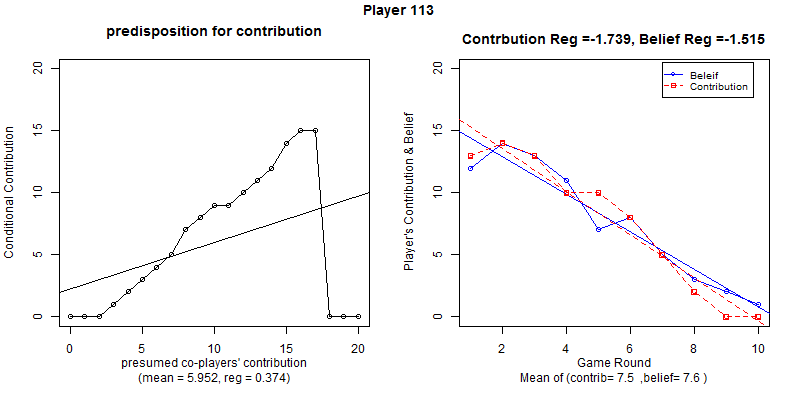
\includegraphics[width=1\textwidth]{images/chapter5/P113.png}
            }\\
            \subfigure{
                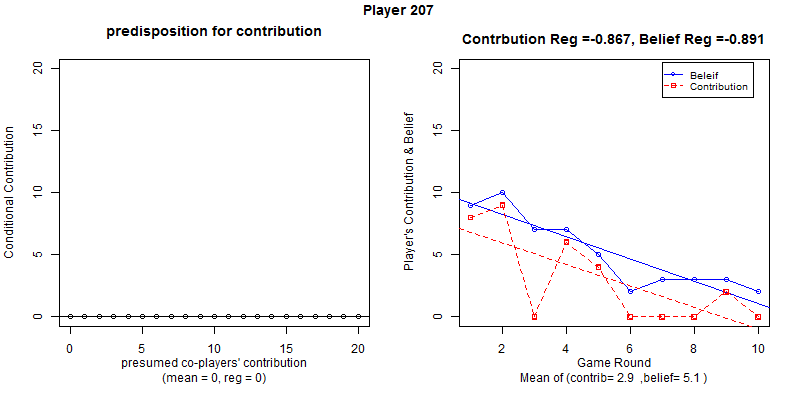
\includegraphics[width=1\textwidth]{images/chapter5/P207.png}   
            }\\
            \subfigure{
                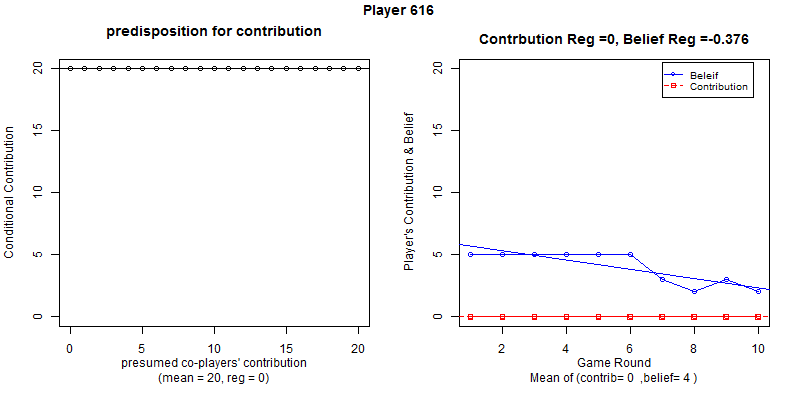
\includegraphics[width=1\textwidth]{images/chapter5/P616.png}
            }\\
        \end{minipage}}
        \caption{Three samples of player's profiles of the public goods game 10 rounds data set.}
        \label{fig:playersProfiles}
    \end{figure}



\subsubsection{Driving Classes from Experts' Knowledge}
Classifying items using human experts' knowledge can be accomplished by two methods. The first method is directly acquiring classes' rules from experts of the field of the data as example \cite{Zadeh1984}. The second method is indirectly driving classes from existing common knowledge about the data and the items which have to be classified. Experts' definition for classes can be used to generate rules. In other cases, rules can be generated from other classification methods as in \cite{Lawrence2001} or numerically analysing the data to generate rules as in \cite{Sugeno1993}. However, in this study, we will combine these two methods to generate initial classes. The rules are derived from a modified version of the available definitions for classes \cite{Fischbacher2001}. To finalise these rules we asked experts iteratively their opinion on the produced classes for players using players' profiles for a visual aid of their decisions. As a reminder for the available classes, we list them here:

\begin{itemize}
    \item \textbf{Conditional Co-Operator:} these players increase their contribution when other players' contribution increases.
    \item \textbf{Free Riders:} these players do not contribute to the project regardless of other players' contribution.
    \item \textbf{Triangle Contributors:} these players' contribution will increase to a point with the rise of other players' contribution to a certain point. Then their contribution starts to decline a while other players increase their amount of contribution.
    \item \textbf{Others:} these players are contributing in a random and unexpected pattern.
\end{itemize}

The above experts' definitions for public goods game players are based on the static data of (contribution table) \cite{Fischbacher2010}. Therefore, we worked closely with 
Professor Gaechter \footnote{\textbf{Simon Gaechter}: School of Economics, the University of Nottingham} and
Doctor Kolle \footnote{\textbf{Felix Kolle}: School of Economics, the University of Nottingham}
to present a modified version of definitions with the aid of visual profiling of players' behaviour across all rounds of the game. 
  

From the visual profiling, we concluded that the behaviour of members of class \textbf{others} do not reflect their actual contribution. This means despite the randomness of their answers in contribution-table the learning factor is affecting their behaviour so that they behaviour become more predictable and follows one of the known classes so that we removed this class for the temporal classification. The visual profiling for the \textbf{triangular contributor} also shows that there is no correlation between players answers in contribution table and their later behaviour in the game rounds so that we removed this class too. As it is known (please see chapter three) that the conditional contributor's class is a large class and contain slightly different behaviours which can all be considered as conditional so that this class is divided into three smaller classes which they are weak contributors, normal contributors and strong contributors. The modified version of classes for players' classes in the public goods game with 20 points as the maximum available contribution points are:

\begin{itemize}
    \item \textbf{Free Riders:} players who contribute by equal or less than one point on average for all rounds or who are not contributing in most rounds. This class corresponds to the traditional category of Free Riders. 
    \item \textbf{Weak Contributors:} players who contribute between 1 and 5 or those not contributing in half of the rounds. In the old categorization, this class loosely relates to conditional contributors.
    \item \textbf{Normal Contributors:} players who contribute on average around 5 points. This class is strongly related to conditional contributors as it fits the same criteria.
    \item \textbf{Strong Contributors:} players who contribute more than 10 points on average. This class relates to conditional comparators and others in the classical categories.
\end{itemize}

However, these class definitions can be vague and lead to imprecise decisions for the final limits of classes. Hence generating imprecise rules for the classes or as described by L. Zadeh \cite{Zadeh1984} ''Much of the uncertainty in the knowledge base of a typical expert system derives from the fuzziness and incompleteness of data, rather than from its randomness''. To overcome this imprecision the [min, max] range of each class limit is proposed as described earlier. 



\begin{table}[!h]
    
    \small
    \centering
    \caption{The attributes' [min, max] values for classification rules}
    \label{tab:minMaxPGGBothDataSets}
    \begin{tabular}{@{}cccccccccccc@{}}
        \toprule
        &    & \multicolumn{3}{c}{\textbf{$\overline{Contribution}$}} &  \phantom{abc}& \multicolumn{3}{c}{\textbf{$\overline{Belief}$}} &  \phantom{abc}& \multicolumn{2}{c}{\textbf{$\left |Zero\right |$}} \\
        
        \cmidrule{3-5} \cmidrule{7-9} \cmidrule{11-12}
        
        &    & FR                & WC                & NC    & \phantom{abc}           & FR              & WC              & NC     & \phantom{abc}        & FR                        & WC                        \\ \midrule
        
        
        \multirow{2}{*}{\begin{turn}{90}{\scriptsize 10 Rounds}\end{turn}}    
        & Min & 
        0                 & 1                 & 2     & \phantom{abc}           
        & 2               & 4               & 2      & \phantom{abc}        
        & 6                         & 5                         \\
        
        &Max & 
        1                 & 4                 & 6     & \phantom{abc}           
        & 9               & 9               & 9       & \phantom{abc}       
        & 9                         & 7\\
        
        \midrule
        
        \multirow{2}{*}{\begin{turn}{90}{\scriptsize 27 Rounds}\end{turn}}
        & Min & 
        0                 & 1                 & 2     & \phantom{abc}           
        & 2               & 4               & 2      & \phantom{abc}        
        & 20               & 15                         \\
        
        &Max & 
        1                 & 4                 & 6     & \phantom{abc}           
        & 9               & 9               & 9       & \phantom{abc}       
        & 25              & 20\\
        
        \bottomrule                        
    \end{tabular}
\end{table}

For the two public goods game data sets used in this experiment, the [min, max] boundaries are determined using the above definitions with multiple iterations of classification to enhance boundaries through domain experts' decisions. The initial boundaries of the classes are an average of the cutting lines between own contribution and others contribution as shown in figure \ref{fig:estimate}. The classification rules are prioritised so that the Free Rider FR class has the highest priority followed by Weak Contributor WC, then Normal Contributor NC while Strong Contributor has the lowest priority. The attribute boundaries for classes are distributed so that all values from the lowest to highest values are covered. This means there are no rules for SC class as players who are not classified with higher priorities will be classified as SC by the 'else' statement. Table \ref{tab:minMaxPGGBothDataSets} shows these range boundaries for attributes which are used to classify players in the public goods game data sets. It can be noticed that the boundaries for both 10 and 27 rounds data sets are similar except for the number of zero contributions, which is different due to the different lengths of the games. The second step of classification will reduce these ranges into scalar values by using optimisation as detailed in the next section.

\begin{figure}[!h]
    \centering
    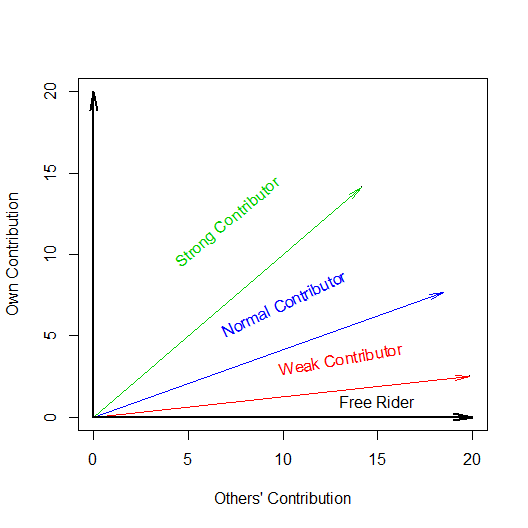
\includegraphics[width=0.8\textwidth]{images/chapter5/estimate.png}
    \caption{Initial estimated range of values of each class.}
    \label{fig:estimate}
\end{figure}


\subsection{Selecting Best Classifier}
\label{sec:Selecting-Best-Classifier}
By selecting a single value from each proposed [min, max] range for the classification rules, we can create a classifier with defined crisp edges. However, the initial classification rules with the proposed range of values for each attribute produce numerous slightly different crisp classification rules. As mentioned in chapter three section  \ref{sec:Optimising-Initial-Rules}, the best classifier will produce the most compacted classes for items at each time point. The compactness of classes is calculated by this equation which we use as a cost function with the aim of minimising it.

\begin{equation}
f(C) = \sum_{t=1}^{T} \sum_{n=1}^{N} CM(c_{n}^{t}) \times \left | c_{n} \right |
\end{equation}

In this function T represents the number of available time points, N is the number of clusters,  $\left | c_{n} \right |$ is the cardinality number of items in cluster n, and $CM(c_{n}^{t})$ is a \gls{CompactMeasure} for cluster n in t time point.

There are many ways to measure the compactness of classes such as Euclidean distances between items, statistical measures, and internal clustering validity measures. To use all of these different compactness measures a general cost function is created with the place holder for the compact measure function as shown in Algorithm \ref{alg:generalCostFunction}. 

However, not all the presented compactness measures can calculate multivariate data such as standard deviation. For this reason, another general function is created to calculate the sum of individual attributes to ensure that all compactness measures can operate in multivariate temporal data. In the next subsections, we will discuss each type of compactness measure.


\begin{algorithm}[!h]
    \SetAlgoLined
    \Fn{cost}{
        \KwIn{CM = Compactness function}
        \KwIn{Temporal data with classification informarion}
        \ForEach{t in Times}{%
            \ForEach{c in Classes}{%
                costs.append(\textbf{CM}(c[t]) * count(c))\;
            }
        }
    }
    
    \caption{General cost function with a place holder for different types of compact measures \textbf{CM}}
    \label{alg:generalCostFunction}
\end{algorithm}



\subsubsection{Statistical Measures}

There are many statistical measures which can calculate the compactness of a single variate data \cite{Watt2002}. There are also other variations of these measures which can analyse multivariate data sets \cite{Harvey1994}. However, we preferred to use the former as they are more widely used and have built-in implementations in most programming languages. For multivariate temporal data sets, we simply calculate the total sum of all single temporal attributes as the final cost function.

For the tests of statistical measures as cost functions, we used standard deviation \textbf{sd} and interquartile range \textbf{IQR}. Sd calculates the dispersion of data around the mean  \cite{Watt2002}. This measure assumes normality of data, so it is not always possible for it to be used as a cost function.   IQR is the distance of the middle 50\% of data which lies between the first and last quarter  \cite{Ross2010}. As this measure ignores the first and fourth quartiles,  it is insusceptible to outlier values. On the other hand, it might ignore them all together which also might not be a desired characteristic. These two statistical functions are not tailored specifically to calculate compactness of data, but they can capture the magnitude of data spread.

\subsubsection{Euclidean Distance}

Euclidean distance is the shortest length between any two points \cite{Deza2009}. Euclidean distance can calculate the distance of two points n and m from one dimension to any D dimension using this equation: 

\begin{equation}
len(n, m) = \sqrt{\sum_{i = 1}^{D} (n_i - m_i)^2}
\end{equation}

To compare results of Euclidean distance based cost function with the statistical results we use the naive method in our experiments as described by Keogh et al. \cite{Keogh2003}. In this method, the total sum of distances for each dimension is calculated by simply looping through all dimensions separately. This loop will change the Euclidean equation to:
\begin{equation}
len(n, m) = \sum_{i = 1}^{D} \sqrt{ (n_i - m_i)^2}
\end{equation}

We used two cost functions based on Euclidean distance. The first cost function is '\gls{CompleteDistance}' which is the total distance of each item in any class to all other items in the same class. The second cost function is 'centroid distance' which is the total distance of items in one class to the centre of that class. This method uses a similar technique which exists in k--means clustering to find the best clusters. Therefore, it may have the same drawbacks of k--means clustering including its sensitivity to extreme values (or outliers) \cite{Wu2002}.


\subsubsection{Internal Cluster Validity Indices}

Internal cluster validity indices are a range of measures designed specifically to validate the results of clustering algorithms using structural information of the proposed clusters by the algorithm. The structure of the clustering includes both 1) compactness of clusters. That is, how close items are to each other inside one cluster and 2) separation between clusters which means how far each cluster is from other clusters. A better clustering algorithm generates closer items in each cluster and more distant clusters from each other \cite{Liu2010}. Please refer to chapter two for more detail on Internal cluster validity indices.

While most of the Internal cluster validity indices are specially designed to measure the compactness of clusters, they calculate the distances of items in the clusters and the distance between clusters at the same time \cite{Zaki2014} and then returns a single value to describe the status of the clusters. While this feature is proven to be important to validate the quality of clustering, it also creates a challenge for embedding them in our cost function which requires multiplying compactness of the cluster to its size. So for our tests with Internal cluster validity indices, we will use a modified version of the proposed cost function which is:
\begin{equation}
f(C) = \sum_{t=1}^{T} \sum_{n=1}^{N} CM(c_{n}^{t}) 
\end{equation}

This modified cost function does not multiply Compactness Measures CM function with $\left | c_{n} \right |$ this might lead the algorithm to create only one or two big clusters. This characteristic of the Internal cluster validity indices might limit their use as CM in our cost functions.

There are many available Internal cluster validity indices \cite{JegathaDeborah2010}. However, for the experiments of the proposed classification method, we selected four Internal cluster validity indices which directly calculate compactness of items in the clusters:

\begin{itemize}
    
    \item Dunn Index (Dunn): is calculated as a ratio of the minimum distance between items of different clusters and maximum distance between items inside a cluster \cite{Dunn1973a}. 
    
    \item Davies.Bouldin (DB): is calculated as the average of all clusters' maximum variance around the mean of their cluster. \cite{Davies1979a}
    
    \item SD: is calculated by using the average scattering of items in each cluster and the total separation between clusters \cite{Halkidi2002}.
    
    \item S\_Dbw: is calculated by using intra-cluster variance and inter-cluster density to identify very compact clusters with the highest separation between clusters \cite{Halkidi2002}. 
\end{itemize}

In the next section, we will compare our results with economists classification to determine the performance of the proposed method using new derived attributes from available attributes of the 10 round public goods game data set.


\section{Performance of the Proposed Classification}

To test the performance of the proposed classification the ten rounds of public goods game data set are used for comparison. We compare our classification results with the labels of players produced by economists using class definitions provided by Fischbacher et al. \cite{Fischbacher2001} for players' strategy types. However, the data set does not provide a ground truth of player types, so it is challenging to make a direct comparison between two methods. To overcome this issue, we compare both results in two ways:

\begin{itemize}
    \item By comparing players' contribution behaviour of each class in all ten rounds. We can assume that this better classification process will produce more homogeneity, hence more compact contribution, at each time point.
    
    \item By using 75\% of the players' data to build two classifiers for another classification model such as SVM. The first classifier is built by using economists' labels for players and the second using the proposed classes in this study. Then, we predict the remaining players' labels and classes using their respective models. The classifier model with a higher level accuracy to predict players' labels or classes is an indication of a better underlying classification method with more consistent results for players' behaviour. The choice of 75\% training and 25\% test are decided by considering two facts. First, there are sufficient data for the classification model to be set due to the fact there are 10 and 27 rounds of the game and then treating each round as a separate dataset. Second, a sufficient amount of test data is required so that we can determine which classification method performs better.
\end{itemize} 


\subsection{Optimizing Classification Rules}

To compare the proposed temporal rule-based classification method with economists' labels for players the rules have to be optimised so that all ranges of [min, max] discussed in detail in section \ref{sec:Choosing_Initial_Limits_for_Classes} become a single value. All possibilities of the range combinations are enumerated using brute force to find the best classifier. The best classifier is selected according to the proposed cost functions in section \ref{sec:Selecting-Best-Classifier} and its subsections. The base of the cost functions might be a statistical measure (IQR or Stdev), Euclidean distance (Complete or centroid), or internal cluster validity indices (Dunn, DB, SD or S\_Dbw)

Table \ref{tab:bestPGG10DataSets} displays the best values as selected by the optimisation process using different cost functions. After this point, each range can be replaced with a single value. For example, the classification rules which determine whether a player is a free rider or not is provided by the experts are as follows:
{\small
\begin{lstlisting}
if((meanContrib<[0,1] && meanBelief<[2,9]) || zeroContrib>[6,9])
   item = 1
\end{lstlisting}
}
After optimising this rule using one of the cost functions such as IQR it becomes:
{\small
\begin{lstlisting}
if ((meanContrib<1 && meanBelief<2) || zeroContrib>6)
   item = 1
\end{lstlisting}
}



\begin{table}[!h]
    
    \ra{1.3}
    \small
    \centering

    \caption{The attributes' best values for the ranges of the initial classification rules of 10 rounds the public goods game data set using different cost functions.}
    \label{tab:bestPGG10DataSets}
    \begin{tabular}{@{}crcccccccccc@{}}
        \toprule
        &    & \multicolumn{3}{c}{\textbf{$\overline{Contribution}$}} &  \phantom{abc}& \multicolumn{3}{c}{\textbf{$\overline{Belief}$}} &  \phantom{abc}& \multicolumn{2}{c}{\textbf{$\left |Zero\right |$}} \\
        
        \cmidrule{3-5} \cmidrule{7-9} \cmidrule{11-12}
        
        &    & FR                & WC                & NC    & \phantom{abc}           & FR              & WC              & NC     & \phantom{abc}        & FR                        & WC                        \\ \midrule
        
        
        \multirow{2}{*}{\begin{turn}{90}{\scriptsize Statistics}\end{turn}}    
        & IQR & 
        1    & 3   & 5 & \phantom{abc}           
        & 2  & 4   & 2 & \phantom{abc}        
        & 6   & 5                         \\
        
        &Stdev & 
        1   & 1   & 6 & \phantom{abc}           
        & 2  & 4  & 2  & \phantom{abc}       
        & 9  & 6\\
        
        \midrule
            
        \multirow{2}{*}{\begin{turn}{90}{\scriptsize Euclidean}\end{turn}}
        &Complete & 
          1  & 3  & 6   & \phantom{abc}           
        & 2  & 4  & 2   & \phantom{abc}        
        & 7  & 5                         \\
        
        &Centroid & 
          1  & 2  & 2  & \phantom{abc}           
        & 2  & 4  & 2       & \phantom{abc}       
        & 6  & 5\\
        
        
        \midrule

        \multirow{4}{*}{\begin{turn}{90}{\scriptsize ICVI }\end{turn}}
        & Dunn & 
          1  & 3  & 2 & \phantom{abc}           
        & 7  & 7  & 2 & \phantom{abc}        
        & 6  & 6    \\
        
        &DB & 
          1  & 4  & 2 & \phantom{abc}           
          & 2  & 5  & 2 & \phantom{abc}        
          & 5  & 6    \\
        
        & SD & 
          1  & 4  & 6 & \phantom{abc}           
          & 7  & 4  & 2 & \phantom{abc}        
          & 9  & 6    \\
        
        &S\_Dbw & 
          1  & 4  & 4 & \phantom{abc}           
          & 2  & 4  & 2 & \phantom{abc}        
          & 8  & 6    \\
        
        \bottomrule                        
    \end{tabular}
\end{table}

To assess the impact of different cost functions on the classification rules the number of players in each class is calculated and listed in Table \ref{tab:bestPGG10DataSets}. As we anticipated in section \ref{sec:Selecting-Best-Classifier}, the cost functions which are based on internal cluster validity indices produce imbalanced classes with one large class except for SD. This is due to the underlying equation for these Internal cluster validity indices. Moreover, the Euclidean based centroid distance creates an empty class, and stdev also creates imbalanced classes, despite multiplying CM with the cardinality of classes to prevent the creation of a large class. 

These cost functions might be modified to work in different situations with different data sets. Moreover, domain specific cost functions can be crafted to fulfil the requirements of the provided initial rules. For the public goods game, we consider that the remaining three cost functions (IQR, Complete Distance and SD) are the best-suited to be used for classifying players in the data. These cost functions do not allow for big classes to form which might be a result of their mathematical equations rather than similarity of players' behaviour. We will, therefore, only use them for later comparisons for the public goods game data sets.

\begin{table}[!h]
    \small
    \centering
    \caption{Number of players in each class (Cardinality number of classes) in 10 rounds of the public goods game data set using different cost functions.}
    \label{tab:NumberOfClassMembershippGG10}
    \begin{tabular}{@{}crccccccccc@{}}
        \toprule
        &Cost Function & \phantom{abc}  & Fr & \phantom{a} & Wc & \phantom{a} & Nc & \phantom{a} & Sc & \phantom{a} \\
        \midrule
        \multirow{2}{*}{\begin{turn}{90}{\scriptsize Statistics}\end{turn}}
        & IQR           & \phantom{abc} & 46 & \phantom{a} & 22 & \phantom{a} & 22 & \phantom{a} & 50 & \phantom{a}\\
        & Stdev         & \phantom{abc} & 36 & \phantom{a} & 10 & \phantom{a} & 58 & \phantom{a} & 36 & \phantom{a}\\
        
        \midrule
        \multirow{2}{*}{\begin{turn}{90}{\scriptsize Euclidean}\end{turn}}
        & Complete      & \phantom{abc} & 38 & \phantom{a} & 30 & \phantom{a} & 37 & \phantom{a} & 35 & \phantom{a}\\
        & Centroid      & \phantom{abc} & 46 & \phantom{a} & 10 & \phantom{a} & 0  & \phantom{a} & 84 & \phantom{a}\\
        
        \midrule
        \multirow{4}{*}{\begin{turn}{90}{\scriptsize ICVI }\end{turn}}
        & Dunn          & \phantom{abc} & 42 & \phantom{a} & 4  & \phantom{a} & 9  & \phantom{a} & 85 & \phantom{a}\\
        & DB            & \phantom{abc} & 37 & \phantom{a} & 34 & \phantom{a} & 2  & \phantom{a} & 67 & \phantom{a}\\
        & SD            & \phantom{abc} & 28 & \phantom{a} & 48 & \phantom{a} & 28 & \phantom{a} & 36 & \phantom{a}\\
        & S\_Dbw        & \phantom{abc} & 37 & \phantom{a} & 40 & \phantom{a} & 1  & \phantom{a} & 62 & \phantom{a}\\
        \bottomrule
    \end{tabular}
\end{table}

\subsection{Comparing Contribution Behaviour of the Players}

The essence of classifying the strategy of players is to describe their contribution behaviour pattern \cite{Fischbacher2001} because the only attribute which matters at the end of each round is how much a player will contribute and then how this contribution changes in the next rounds. Therefore, any classification which can create more similar players with the same contribution behaviour at each time point is a better classification method. To determine which classification method performs better at classifying players' according to their behaviour, we compare each class's contribution distribution at each time point for both our proposed classification and the available classification for the public goods game. 

We use two methods for comparing the distribution of classes' contribution. The first is to use the visual method of box-plots and means, and the second involves using the average of standard deviation. We compare contribution behaviour of economists' labels against our classification method according to the three selected cost functions.



\begin{figure}[!h]
    \centering
    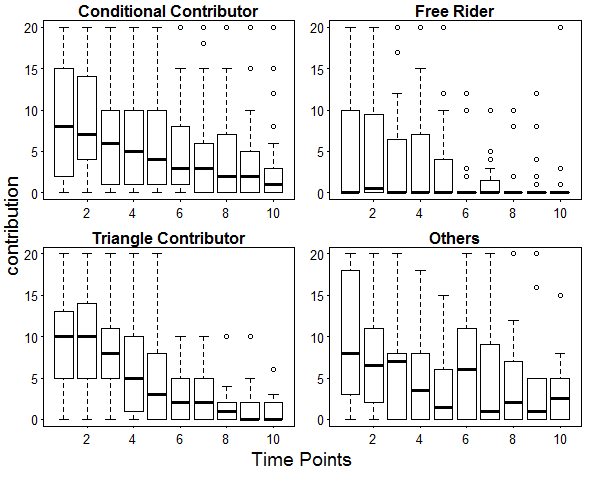
\includegraphics[width=0.8\textwidth]{images/chapter5/economists_PGG10_Boxplot.png}
    \caption{Boxplots of the players' contribution behaviour of different player labels in the 10 rounds data set of the public goods game. The labels are generated using economists' definitions for various strategy types.}
    \label{fig:economists_PGG10_Boxplot}
\end{figure}

Figure \ref{fig:economists_PGG10_Boxplot} shows boxplots of the public goods game players' contribution at all time points (rounds) for each label of players separately. Players are classified using economists method for classifying players which depend on the contribution table (none-temporal attributes). In this figure, we can observe that:

\begin{itemize}
    \item The median of free riders is almost always zero (except round two). However, the first five rounds show a very high IQR values which can be interpreted as there is a large difference in players' behaviour. 
    
    \item The median of the players' contribution is gradually dropping as expected. However, all rounds have a large value for IQR, which might be an indication that player strategy varies from contribution table to and actual contributions.
    
    \item There is no significant difference between behaviours of triangular contributors and conditional contributors except starting with a little higher contribution, and there is a steeper drop for it during the rounds.
    
    \item The others class players do not follow any pattern for their contribution.
\end{itemize}


\begin{figure}[!h]
    \centering
    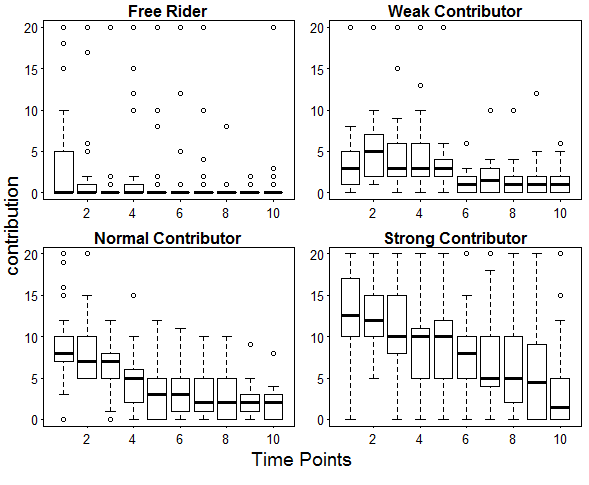
\includegraphics[width=0.8\textwidth]{images/chapter5/IQRCost_PGG10_Boxplot.png}
    \caption{Boxplots of the players' contribution behaviour in different classes which are generated using proposed classification method with IQR as a CM for the cost function.}
    \label{fig:IQRCost_PGG10_Boxplot}
\end{figure}

\begin{figure}[!h]
    \centering
    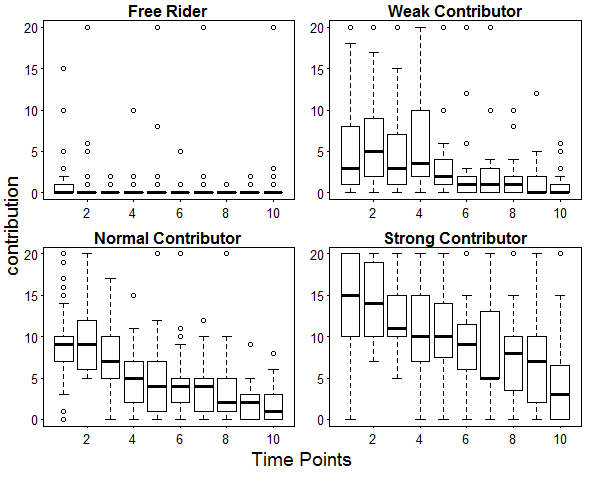
\includegraphics[width=0.8\textwidth]{images/chapter5/ColpleteCost_PGG10_Boxplot.png}
    \caption{Boxplots of the players' contribution behaviour in different classes which are generated using proposed classification method with Euclidean complete Dist. as a CM for the cost function.}
    \label{fig:ColpleteCost_PGG10_Boxplot}
\end{figure}

\begin{figure}[!h]
    \centering
    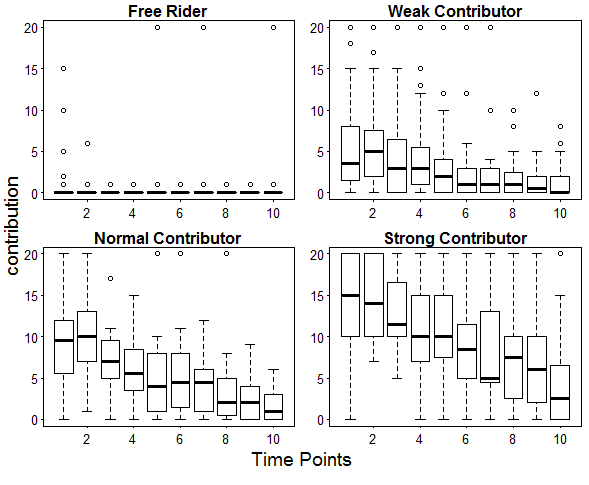
\includegraphics[width=0.8\textwidth]{images/chapter5/SDCost_PGG10_Boxplot.png}
    \caption{Boxplots of the players' contribution behaviour in different classes which are generated using proposed classification method with SD as a CM for the cost function.}
    \label{fig:SDCost_PGG10_Boxplot}
\end{figure}


Figures \ref{fig:IQRCost_PGG10_Boxplot}, \ref{fig:ColpleteCost_PGG10_Boxplot} and \ref{fig:SDCost_PGG10_Boxplot} show the public goods game players' contributions boxplots for different classes using proposed classification with cost functions IQR, Complete Distance and SD respectively. In these figures, we can observe that:

\begin{itemize}
    \item Free riders' median is always zero with very low IQR values mean that players contribution in these classes is mostly zero as expected.
    
    \item Except for strong contributors, the IQR values for other classes at all time points are lower than economists classes.
    
    \item There is a noticeable difference in the players' contribution median from one class to the next as the contribution of the same time point rises from free rider to weak contributor and so on.
    
    \item Except for the free rider class, all other classes' contribution median gradually drops as expected.
\end{itemize}

According to these observations, we can conclude that the proposed classification method can produce better classes for players according to their behaviour with more homogeneous contributions among the same class. To check these observations, we calculated the average of the standard deviation of the ten rounds for each classes' contribution.


\begin{table}[!h]
    \small
    \centering
    \caption{The ten rounds' average of standard deviation for players' contribution of each class using various cost functions to produce players' classes which are compared with the economist labels.}
    \label{tab:stdevContribDistribution_PGG10}
    \begin{tabular}{@{}rccccccccc@{}}
        \toprule
        Cost Function & \phantom{aa} & FR & \phantom{a} & WC & \phantom{a} & NC & \phantom{a} & SC  & Mean \\
        \midrule
        IQR           & \phantom{aa} & 4  & \phantom{a} & 3.3& \phantom{a} & 3.3& \phantom{a} & 5.5 &  4    \\
        Complete      & \phantom{aa} & 2.1& \phantom{a} & 4.6& \phantom{a} & 3.7& \phantom{a} & 5.6 &  4    \\
        SD            & \phantom{aa} & 1.7& \phantom{a} & 3.9& \phantom{a} & 3.9& \phantom{a} & 5.7 &  3.8  \\
        \midrule
        Economists'-  & \phantom{aa} & CC & \phantom{a} & FR & \phantom{a} & TC & \phantom{a} & OT  &  Mean \\
        Classification& \phantom{aa} & 5.7& \phantom{a} & 4.5& \phantom{a} & 4.2& \phantom{a} & 6.3 &  5.2   \\
        \bottomrule
    \end{tabular}
\end{table}

 Table \ref{tab:stdevContribDistribution_PGG10} shows that the classes of the proposed classification method with different cost functions have smaller standard deviation on average in comparison to the economists' labels for players. This means less spread of contribution at each time point which might be an indication of better class models for the players' actual contribution behaviour.


\subsection{Using Third Classifier for Comparison}

We use a third classification algorithm to compare the proposed classification method and the existing economists' labels. In this experiment, we selected SVM classification as the third classifier due to its proven success and wide acceptance  \cite{Bazi2006}. SVM uses optimised hyperplanes to classify data. Hyperplanes can be linear or nonlinear according to the used kernel in training. These hyperplanes are optimised through training using pre-classified data sets.

Four SVM classifiers are created using 75\% of the players' data and class labels. Each of these classifiers used different labels of players which are originally generated by using either the economists' classification or our proposed classification with different cost functions (IQR, CompleteDist or SD). Then, we used the remaining 25\% of the players to test the accuracy of the different SVM classifiers. The more accurate these classifiers are, the better reliable and consistent labels are presented to them in the training and testing sessions.  Hence, the better classifier has produced the train/test labels in the first place. We used each time point of the public goods game data set separately to avoid a temporal dimension for the SVM classifier and to check how consistent the provided labels are at each time point. Moreover, multiple new attributes are derived from existing attributes and used for the classification to determine the accuracy of the classifiers with attributes which have not been used to generate train/test labels. The new attributes are:

\begin{itemize}
    \item  \textit{Payoff}: The number of points an individual player gathers during each round. This can be calculated by points that they kept + public goods project returns. The payoff value may have a high impact on the players' behaviour for the next rounds.
    
    \item  \textit{$ \overline{ContribTab} $}: The average of 'contribution table' which is indicated by attributes [b0-b20]. This attribute is important in estimating the overall level of players' initial willingness to contribute.
    
    \item  \textit{$ \overline{Contrib} $}: The average of players' contribution in all rounds. This field is important to ascertain the general level of contribution during the game.
    
    \item  \textit{InitialDiff}: Difference between actual contribution and supposed contribution according to the players' contribution table. The importance of this attribute is to determine the amount of players' strategy change during the game rounds.
    
    \item  \textit{$ \overline{initialDiff} $}: Average of \textit{InitialDiff} during all game rounds. This attribute validates player's initial claim of willingness for contribution.
    
    \item \textit{PredecAcc}: Accuracy of players' prediction. This attribute is calculated as the difference between player's belief about other players contribution and their actual contribution.
    
    \item  \textit{PredecAccSD}: Standard Deviation of \textit{PredecAcc} for each player in all rounds of the game. This attribute detects how much a player correctly anticipates their co-players' strategy.
    
\end{itemize}


The new attributes which are derived from existing data may raise concerns about the level of correlation between them as they might affect the performance of the classification. Table \ref{tab:createdAttributeCorelation} addresses all correlation values among these attributes.

\begin{table}[!h]
    \small
    \centering
    \caption {Correlation value among created attributes}
    \label{tab:createdAttributeCorelation}
    \begin{tabular}{r|cccccc}
        \textit{Contrib}   & 0.549  &        &  &        &      &       \\
        \textit{Payoff}                   & -0.135 & -0.58        &  &     &         &       \\
        $ \overline{ContribTab} $  & 0.048  & 0.208        & -0.169 &       &       &       \\
        $ \overline{Contrib} $     & 0.263  & 0.684        & -0.486 & 0.296      &    &       \\
        \textit{InitialDiff}              & 0.235  & 0.511      & -0.285 & 0.251   & 0.361  &       \\
        $ \overline{initialDiff} $ & 0.097  & 0.332      & -0.218 & 0.34   & 0.489   & 0.743    \\ \hline
        & \textit{Belief} & \textit{Contrib} & \textit{Payoff} & $ \overline{ContribTab} $ & $ \overline{Contrib} $ & \textit{InitialDiff} \\ 
    \end{tabular}
\end{table}


The average of AUC of ROC analysis is used to measure the accuracy of the SVM classifiers. To train the classifiers and then test their accuracies different attribute sets are used to create these classifiers. The first set is both contribution and belief of players, the second is original attributes of players, the third attribute set is the derived attributes above, and the last attribute set contains all available attributes.

The accuracy results of the SVM classifier with different sets of attributes and different classes for players are shown in Table  \ref{teb:AUCofSVMTest}. It can be noticed that the SVM classifier for all proposed classes with different cost functions perform better than economists' labels for players in predicting the test set except in the case of IQR cost function when original attributes are used. Moreover, the SVM classifier is more accurate for all attribute sets using proposed classes with SD cost function. This result aligns with the previous test results of the players' contribution behaviour compactness in each time point as the SD cost function produced the most compacted behaviours with minimum standard deviation.

The results of the last two tests indicate that the proposed temporal classification method with different cost functions can classify players better than the available method which means Hypothesis \ref{hypo:proposedClassification} holds true. Various cost functions and initial ranges for classification rules provide more flexibility so that the best classifier can be selected for the temporal items. We showed that, by combining human expertise and computer optimisation, we can create better classes than the domain specific classifier, yet with simple rules which can be understood by experts. Rule simplicity is a positive point in this classifier as it allows experts to adjust their initial rules further to create better classes in a reiterated classification. Simple rules might be necessary to gain a better understanding for items behaviour in the underlying complex temporal data.


\begin{table}[!h]
    \ra{0.9}
    \small
    \centering
    \caption{Mean of AUC for SVM using different attribute sets to compare proposed classification and existing labels}
    \label{teb:AUCofSVMTest}
    \begin{tabular}{rcccccc}
        \toprule
        \multicolumn{1}{c}{\multirow{2}{*}{Attributes}} & \phantom{a} & Economists' & \phantom{a} & \multicolumn{3}{c}{Proposed Classes} \\
        \cmidrule{5-7}
        \multicolumn{1}{c}{}  & \phantom{a} & labels   & \phantom{a}     & IQR       & Complete     & SD        \\
        \midrule
        Belief+Contrib    & \phantom{a}  & 0.497     & \phantom{a}    & 0.755     & 0.787        & 0.798     \\
        Original  & \phantom{a} & 0.723  & \phantom{a}       & 0.685     & 0.758        & 0.768     \\
        Derived    & \phantom{a} & 0.650  & \phantom{a}       & 0.824     & 0.832        & 0.861     \\
        All  & \phantom{a} & 0.703  & \phantom{a}       & 0.726     & 0.790        & 0.814    \\
        \bottomrule
    \end{tabular}
\end{table}


\section{Analysing the Behaviour of Public Goods Games Players}



After successfully testing and comparing the proposed classification method with the existing method of classifying players of public goods game, we will use created classes through this method to study players' behaviour further. In this section, we will conduct two more analyses. First, we will compare both public goods game data sets players to determine the effect of the game's length on the players' behaviour. Second, we will use players' classes as the reference of behaviour for measuring their behaviour change over time.

\subsection{Players' Strategy in Different Lengths of the Game}
To determine the effect that the duration of the game rounds may have on the players' behaviour and to check the validity of Hypothesis \ref{hypo:lengthOftheGame}, we compare players' class membership from both public goods game data sets (10 and 27 rounds). If both data sets produce comparable class memberships, then the number of rounds may not affect the players. Otherwise, players' behaviour may change due to the longer game rounds. 

In this experiment, we will classify players of 27 rounds data set of public goods game and then compare the cardinality number of classes with players of 10 rounds game using Wilcoxon-test. We will compare the class cardinality of the proposed classes of all three selected cost functions (IQR, Complete Distance and SD). If the samples from the experiments are considered to have the same population mean rank, then there might be no effect of the length of the game on the players' behaviour.

Before starting the comparison, the initial rules of section \ref{sec:Choosing_Initial_Limits_for_Classes} for 27 rounds of the public goods game are optimised using the same brute force method as the 10 rounds game. The results of the best values for the ranges of the rules are shown in Table \ref{tab:bestPGG27DataSets}. The cardinality number of each class is given in Table \ref{tab:NumberOfClassMembershippGG27}. It can be noticed that the SD cost function creates imbalanced classes. This means that, despite the best results which are produced by SD in the 10 rounds of the public goods game data set, it is specific to that particular data. The SD result indicates that our initial prediction about the internal classification indices was accurate as they may produce imbalanced and empty classes. However, as SD cost function proved its ability to perform well in specific situations, they can, therefore, be used for specific data sets if they can fit them.


\begin{table}[!h]
    \ra{1.3}
    \small
    \centering
    
    \caption{The attributes' best values for the ranges of the initial classification rules of 27 rounds of the public goods game data set using selected cost functions.}
    \label{tab:bestPGG27DataSets}
    \begin{tabular}{@{}rcccccccccc@{}}
        \toprule
        & \multicolumn{3}{c}{\textbf{$\overline{Contribution}$}} &  \phantom{abc}& \multicolumn{3}{c}{\textbf{$\overline{Belief}$}} &  \phantom{abc}& \multicolumn{2}{c}{\textbf{$\left |Zero\right |$}} \\
        
        \cmidrule{2-4} \cmidrule{6-8} \cmidrule{10-11}
        
        & FR                & WC                & NC    & \phantom{abc}           & FR              & WC              & NC     & \phantom{abc}        & FR                        & WC                        \\ \midrule

        IQR & 
        1    & 3   & 3 & \phantom{abc}           
        & 2  & 4   & 2 & \phantom{abc}        
        & 20   & 15                         \\
        
        Complete & 
        1  & 1  & 3   & \phantom{abc}           
        & 3  & 4  & 2   & \phantom{abc}        
        & 24  & 17                         \\
        
        
        SD & 
        1  & 4  & 6 & \phantom{abc}           
        & 4  & 9  & 2 & \phantom{abc}        
        & 20  & 20    \\
        
        \bottomrule                        
    \end{tabular}
\end{table}


We used each classes' percentage for comparison purposes between two different data sets as they do not contain the same number of players. The p-value of Wilcoxon-test equals 0.4942, which suggests that the null hypothesis is true and the two samples have the same population mean Rand. This might be an indication that the duration of the game does not affect the players' strategy. Moreover, this result is aligned with our findings in chapter four that the behaviour of the players in both data sets is consistent.

\begin{table}[!h]
    \small
    \centering
    \caption{Number of players in each class (Cardinality number of classes) in 27 rounds of the public goods game data set using different cost functions.}
    \label{tab:NumberOfClassMembershippGG27}
    \begin{tabular}{@{}rccccccccc@{}}
        \toprule
        Cost Function & \phantom{abc}  & Fr & \phantom{a} & Wc & \phantom{a} & Nc & \phantom{a} & Sc & \phantom{a} \\
        \midrule

        IQR           & \phantom{abc} & 48 & \phantom{a} & 29 & \phantom{a} & 31 & \phantom{a} & 20 & \phantom{a}\\

        Complete      & \phantom{abc} & 67 & \phantom{a} & 29 & \phantom{a} & 14 & \phantom{a} & 18 & \phantom{a}\\
    
        SD            & \phantom{abc} & 63 & \phantom{a} & 1 & \phantom{a} & 61 & \phantom{a} & 3 & \phantom{a}\\

        \bottomrule
    \end{tabular}
\end{table}

\subsection{New Players Classes' as Reference of Behaviour}

After players were classified according to their temporal attributes which reflect their contribution behaviour, we can use the new players' classes as a reference of behaviour to check the validity of Hypothesis \ref{hypo:overallBehavoiur}. In chapter four, we examined two different reference of behaviours; the first time point as a reference of behaviour and the previous time point. In this section, we will continue with the last proposed reference of behaviour, which is players' universal behaviour during the game. As the proposed classification uses aggregations of temporal attributes to create classification rules and then optimises them through each time point of the temporal data,  it is, therefore,  suitable to be used as a general (universal) reference of behaviour for players.

As shown in Figures \ref{fig:test_ChangeMeasuers_Class_PGG10} and \ref{fig:test_ChangeMeasuers_Class_PGG27}, there are significant differences between players' classes and the their temporal behaviour. This difference can be seen with the low value of the behavioural change measures across all clusterings and all different external cluster validity indices (less than 0.6). This indicates that the players do not always employ the same strategy. Instead, they try and explore other strategies which contribute to their learning process to different strategy results. However, the regression of the behavioural change for all cases is small (near zero), which indicates the difference is stable throughout all time points. This is another indication that, despite their temporary strategy change, these changes do not affect their general behaviour when playing. 



        \begin{figure}[!h]
            \hfill\begin{minipage}{\dimexpr \textwidth-2\fboxsep-2\fboxrule}% maximum allowed
                    \centering
                    \subfigure[K--means Clustering]{
                        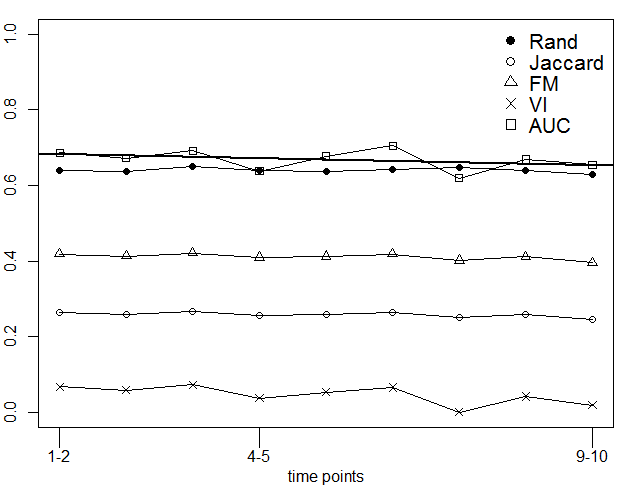
\includegraphics[width=0.45\textwidth]{images/chapter5/Kmeans_class_refPoint_PGG10.png}
                    }
                    \subfigure[PAM Clustering]{
                        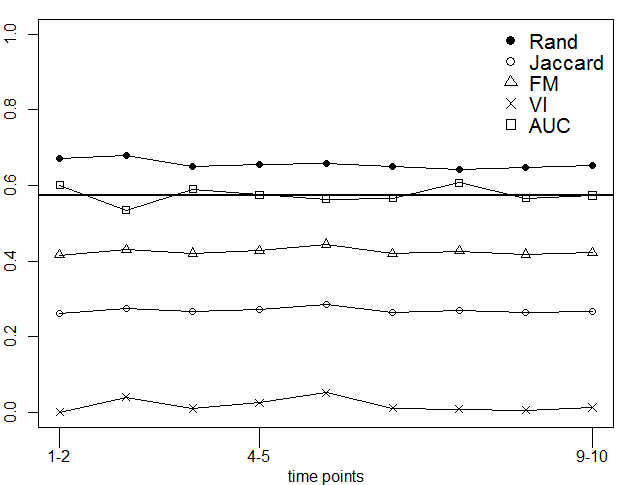
\includegraphics[width=0.45\textwidth]{images/chapter5/PAM_class_refPoint_PGG10.png}
                    }\\
                    
                    \centering
                    \subfigure[C--means Clustering]{
                        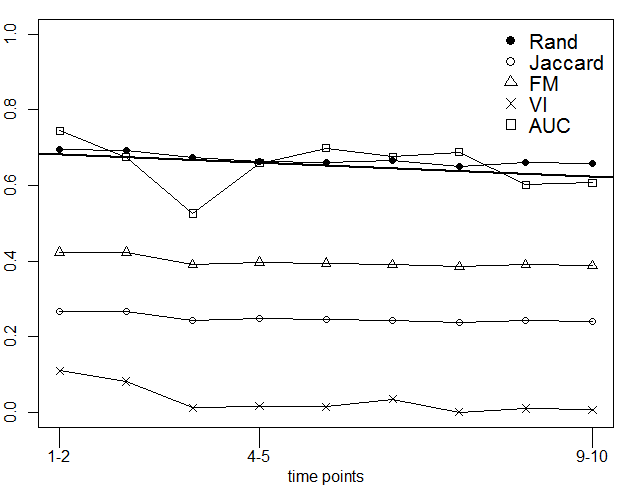
\includegraphics[width=0.45\textwidth]{images/chapter5/Cmeans_class_refPoint_PGG10.png}
                    }
                    \subfigure[Hierarchical Clustering]{
                        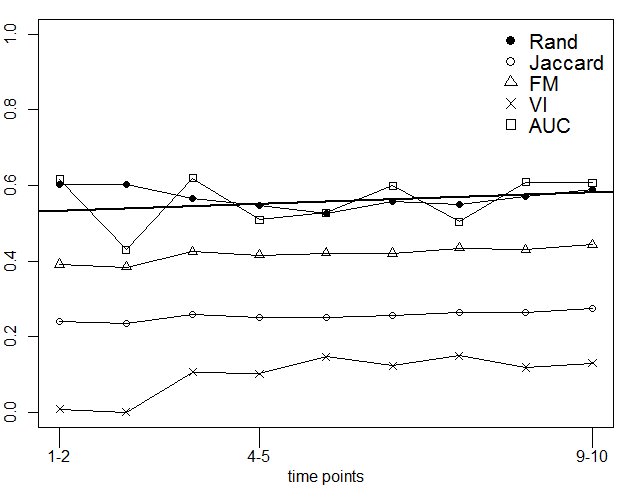
\includegraphics[width=0.45\textwidth]{images/chapter5/hclust_class_refPoint_PGG10.png}
                    }\\
                    
                \end{minipage}            
                \caption{Results of various clustering methods using proposed classes as a reference of behaviour to calculate the magnitude of changes which happen to the groups of items in consequent time points in the test dataset. The amount of change  is measured by using different external cluster validity indices and AUC of ROC.}
                \label{fig:test_ChangeMeasuers_Class_PGG10}
            \end{figure}

Despite the sensitivity difference between external cluster validity indices, all the results of different clusterings and external cluster validity indices are similar to regression slope being equal to zero. This might be an indication that using items' overall general behaviour in the temporal attributes can create more stable predictions than other two reference of behaviours on the items' behavioural change. However, each reference of behaviour can be useful for certain situations. This means that Hypothesis \ref{hypo:overallBehavoiur} holds true. Using the first time point as the reference of behaviour will demonstrate how items are deviating from their initial behaviour. Using the previous time point shows the stability of the items during different stages of the temporal data. Using players' temporal classes as the reference of behaviour demonstrates items behavioural variability in various stages related to their overall behaviour across all time points.


        \begin{figure}[!h]
            \hfill{\begin{minipage}{\dimexpr \textwidth-2\fboxsep-2\fboxrule}% maximum allowed
                    \centering
                    \subfigure[K--means Clustering]{
                        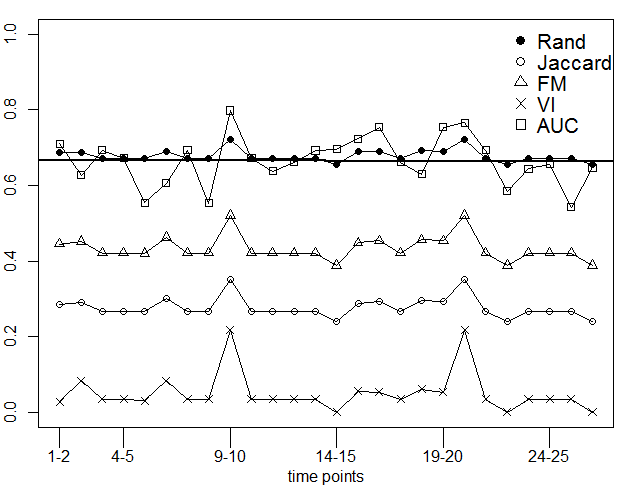
\includegraphics[width=0.45\textwidth]{images/chapter5/Kmeans_class_refPoint_PGG27.png}
                    }
                    \subfigure[PAM Clustering]{
                        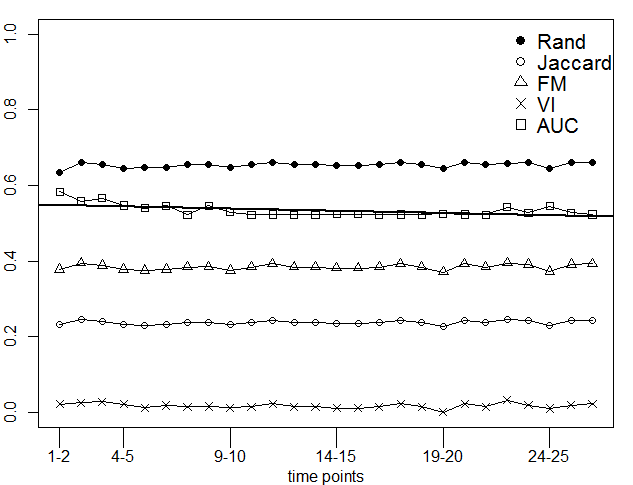
\includegraphics[width=0.45\textwidth]{images/chapter5/PAM_class_refPoint_PGG27.png}
                    }\\
                    
                    \centering
                    \subfigure[C--means Clustering]{
                        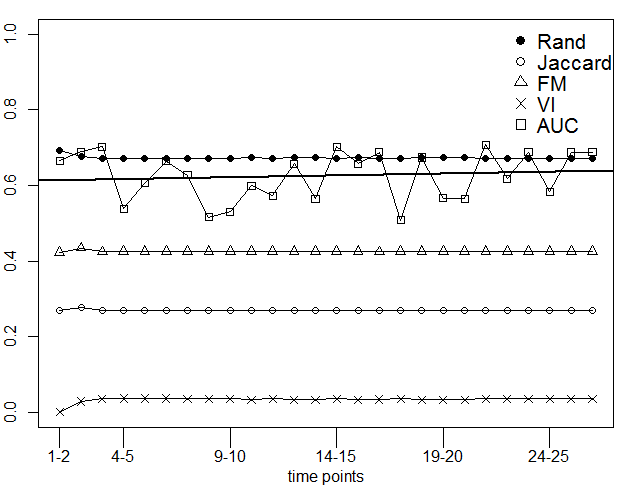
\includegraphics[width=0.45\textwidth]{images/chapter5/Cmeans_class_refPoint_PGG27.png}
                    }
                    \subfigure[Hierarchical Clustering]{
                        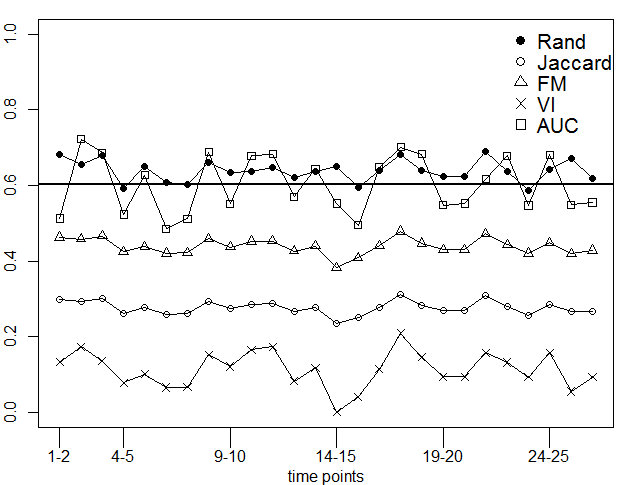
\includegraphics[width=0.45\textwidth]{images/chapter5/hclust_class_refPoint_PGG27.png}
                    }\\
                    
                \end{minipage}}
                \caption{Results of various clustering methods using proposed classes as the reference of behaviour to calculate the magnitude of changes which happen to the groups of items in consequent time points in the test dataset. The amount of change  is measured by using different external cluster validity indices and AUC of ROC.}
                \label{fig:test_ChangeMeasuers_Class_PGG27}
            \end{figure}



\section{Summary} 

In this chapter, we answered the three questions posed in chapter one. The first question concerned the ability to classify players of public goods game to use their temporal attributes during the game rounds. The other two questions were dependent on the first question as temporal classes of the players were required to answer the remaining two questions regarding players' behaviour in the public goods game.

To answer the first question, we proposed a rule-based temporal classification method as mentioned in chapter three section  \ref{sec:Temporal-Rule-Based-Classification}. The proposed classification is based on optimising rules which are provided by human experts. For the sake of simplicity, these rules are generated through aggregating the temporal attributes so that domain experts can handle and understand them. The provided rules contain ranges of values which have to be optimised to create the best compacted classes of items at each time point.

To optimise the initial rules we used brute force to enumerate all possibilities and find the best classifier. The best classifier is determined through a cost function which assures the most compacted classes in each time point. We tested multiple compactness measures \textbf{CM} in the optimisation process including statistical, Euclidean distance and internal clustering validity indices. The best CM were IQR and the complete Euclidean distance between items. As we anticipated, all the  Internal cluster validity indices except for SD in one situation (with 10 rounds of the public goods game) were proven to create large imbalanced classes, as their cost function could not adjust the size of the groups. This was not a concern for the original use of these measures.

To check the validity of Hypothesis \ref{hypo:proposedClassification}, we classified the players of the ten rounds of public goods game data set with the new proposed classes. Then, we compared the new classes of players with the labels provided by economists in two ways. First,  by comparing the contribution behaviour of the players in each class and label for all ten rounds. We used IQR and standard deviation 'stdev' to measure the spread of players contribution in the classes at each time point. For all cases, our proposed classes created more similar behaviours among players of the same class than the economists' labels. Second, we trained SVM classifier using our classes and economists' labels with 75\% of the players and tested them to determine the rest of the players at each time point. The results showed that the SVM classifiers, which are trained with the proposed classes, could detect the classes of the rest of players with a higher level of accuracy than the classifier which is trained and tested using existing players' labels. The results of both tests indicate that the proposed classification method can produce better classes for players of PGG than the available method.

To answer the second question, which concerns players behaviour in different length of public goods game, and to validate Hypothesis \ref{hypo:lengthOftheGame} which suggests that there is no effect of the games' duration on players behaviour. We classified 27 rounds of the public goods games data set and compared the percentage of players in each class with the 10 rounds of public goods game. We determined that there is no significant difference between the two samples which proves the validity of Hypothesis \ref{hypo:lengthOftheGame}. Moreover, a closer examination of the optimised rules shows that these rules are not identical. However, they are close to each other and similar especially if we rule out the differences which are mainly caused by the duration of the game, such as the number of zero contributions.

To answer the last question about the overall behaviour change of the players, we used the produced players' classes of both data sets as the reference of behaviour. The results for both data sets indicate that the players' change over time is stable with near zero regression for all different measures using different clustering methods. This proves that Hypothesis \ref{hypo:overallBehavoiur} holds true.

In the next chapter, we will classify a larger data set of stock market using our proposed classification method. To reduce the time required for the optimisation process, we will use a heuristic method called differential evolution.


